\documentclass[8pt]{beamer}
\usetheme{Copenhagen}
\usecolortheme{dolphin}
\usepackage{a4wide}
\usepackage{epsfig}
\usepackage{amsmath}
\usepackage{tabu}
\usepackage{amsfonts}
\usepackage{latexsym}
\usepackage[utf8]{inputenc}
\usepackage{listings}
\usepackage{color}
\usepackage{titlesec}    
\usepackage{enumitem}
\usepackage[catalan]{babel}
\usepackage{newunicodechar}
\usepackage{graphicx}
\usepackage{subcaption}
\usepackage{float}
\usepackage[numbered,framed]{matlab-prettifier}
\usepackage{xcolor}
\usepackage{pgf, tikz}
\usepackage{listings}
%% listings-modelica.cfg
%% Copyright 2014 Martin Sjoelund, Dietmar Winkler
%
% This work may be distributed and/or modified under the
% conditions of the LaTeX Project Public License, either version 1.3
% of this license or (at your option) any later version.
% The latest version of this license is in
%   http://www.latex-project.org/lppl.txt
% and version 1.3 or later is part of all distributions of LaTeX
% version 2005/12/01 or later.
%
% This work has the LPPL maintenance status `maintained'.
%
% The Current Maintainer of this work is Dietmar Winkler
%
% Code repository https://github.com/modelica-tools/listings-modelica
%
% This work consists of the file listings-modelica.cfg

\lstdefinelanguage{modelica}
{
  morekeywords=[1]{
    algorithm,and,annotation,as,assert,block,break,case,class,connect,connector,
    constant,constrainedby,der,discrete,each,else,elseif,elsewhen,encapsulated,
    end,enumeration,equality,equation,expandable,extends,external,failure,final,
    flow,for,function,guard,if,import,in,initial,inner,input,List,local,loop,
    match,matchcontinue,model,not,operator,Option,or,outer,output,package,parameter,
    partial,protected,public,record,redeclare,replaceable,return,stream,
    subtypeof,then,Tuple,type,uniontype,when,while},
  morekeywords=[2]{true, false},
  % Do not make true,false keywords because fn(true,x, false ) shows up as fn(true,x, *false*)
  morekeywords=[3]{optimization,constraint}, % Optimica keywords
  morekeywords=[4]{objective,startTime,finalTime,initialGuess},
  sensitive=true,
  comment=[l]//,
  morecomment=[s]{/*}{*/},
  alsodigit={.,-},
  morestring=[b]',
  morestring=[b]",
}[keywords,comments,strings]

\definecolor{keywordcolor1}{rgb}{0,0,.4}
\definecolor{keywordcolor2}{rgb}{.90,0,0}
\definecolor{keywordcolor3}{rgb}{.4,0,.8}
\definecolor{keywordcolor4}{rgb}{0.5,0,0.5}
\definecolor{stringcolor}{rgb}{0.133,0.545,0.133}
% \definecolor{listingbgcolor}{rgb}{0.95,0.95,0.95}

\lstset{
  breaklines=true,
  language=modelica,
  basicstyle=\ttfamily,
  keywordstyle=[1]\color{keywordcolor1}\bfseries,
  keywordstyle=[2]\color{keywordcolor2},
  keywordstyle=[3]\color{keywordcolor3}\bfseries,
  keywordstyle=[4]\color{keywordcolor4},
  stringstyle=\color{stringcolor},
%  backgroundcolor=\color{listingbgcolor},
  framexleftmargin=5pt,
  xleftmargin=5pt,
  xrightmargin=5pt,
  showstringspaces=false
}

\newcommand{\code}[1]{\lstinline|#1|}
\newcommand{\modelica}[1]{\lstinline[language=modelica]|#1|}

\usetikzlibrary{arrows, automata, positioning, datavisualization, datavisualization.formats.functions}

\setcounter{tocdepth}{4}
\setcounter{secnumdepth}{4}

\newunicodechar{Ŀ}{\L.}
\newunicodechar{ŀ}{\l.}

\definecolor{dkgreen}{rgb}{0,0.6,0}
\definecolor{gray}{rgb}{0.5,0.5,0.5}
\definecolor{mauve}{rgb}{0.58,0,0.82}

\geometry{paperwidth=150mm,paperheight=115mm}

\lstset{frame=tb,
language=Matlab,
aboveskip=3mm,
belowskip=3mm,
showstringspaces=false,
columns=flexible,
basicstyle={\small\ttfamily},
numbers=none,
numberstyle=\tiny\color{gray},
keywordstyle=\color{blue},
commentstyle=\color{dkgreen},
stringstyle=\color{mauve},
breaklines=true,
breakatwhitespace=true,
mlscaleinline=false,
basicstyle=\tiny,
tabsize=3,
extendedchars=true,
literate={á}{{\'a}}1 {à}{{\`a}}1 {ã}{{\~a}}1 {é}{{\'e}}1 {è}{{\`e}}1 {í}{{\'i}}1 {ï}{{\"i}}1 {ó}{{\'o}}1 {ò}{{\`o}}1 {ú}{{\'u}}1 {ü}{{\"u}}1 {ç}{{\c{c}}}1
			{Á}{{\'A}}1 {À}{{\`A}}1 {Ã}{{\~A}}1 {É}{{\'E}}1 {È}{{\`E}}1 {Í}{{\'I}}1 {Ï}{{\"I}}1 {Ó}{{\'O}}1 {Ò}{{\`O}}1 {Ú}{{\'U}}1 {Ü}{{\"U}}1 {Ç}{{\c{C}}}1
}

\usepackage{hyperref}
\hypersetup{
  colorlinks=false, %set true if you want colored links
  linktoc=all,     %set to all if you want both sections and subsections linked
  linkcolor=blue,  %choose some color if you want links to stand out
}

\title{Simular i dimensionar un sistema de Service Desk}
\author{Marc Cané \and Ismael El Habri \and Lluís Trilla}

\date[KPT 2004] % (optional)
{12 de Desembre del 2018}
\subject{Computació Numèrica i Simulació}

\AtBeginSection[]
{
  \begin{frame}
    \frametitle{Table of Contents}
    \tableofcontents[currentsection]
  \end{frame}
}
\begin{document}

\frame{\titlepage}

\section{Plantejament del problema}
  \begin{frame}
    \frametitle{Plantejament}
    En el nostre exercici s'ens proposava simular un sistema de Service Desk centralitzat per a una empresa. Hi ha diversos nivells d'empleats, de manera que els nivells inferiors tractaran la majoria d'avaries, i les que no es puguin resoldre es passaran a un nivell superior on el personal tindrà major formació.
    \begin{figure}[h!]
      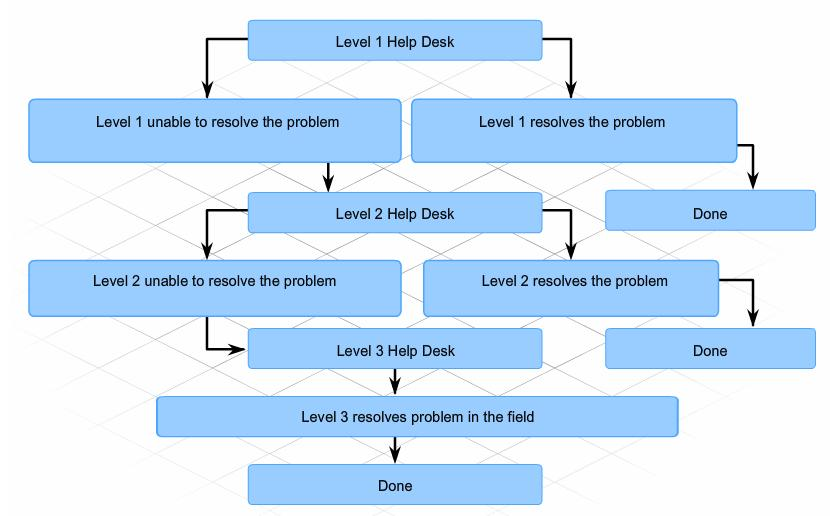
\includegraphics[width=\linewidth]{help-desk-levels.jpg}
      \label{fig:plot1}
    \end{figure}
  \end{frame}
  \begin{frame}
  Per a fer el model hem dissenyat diferents models intermitjos, que ens serviran per simular cada fase del procés:
\begin{itemize}
  \item \textbf{ServiceDesk}: Model que simula tot el sistema de service desk de la empresa.
  \item \textbf{Empresa}: Model que simula la generació d'incidències de l'empresa.
  \item \textbf{Resolució}: Model que simula la resolució d'incidències.
  \item \textbf{UnificadorSolucionades}: Model que rep totes les incidències resoltes i les unifica.
  \item \textbf{incidencies}: Classe connector per transmetre incidències 
\end{itemize}
\end{frame}

\begin{frame}
\section{Model Incidències}
\lstinputlisting[language=modelica]{../Incidencies.mo}

Aquesta classe no te cap secret, és de tipus connector i té un element Real \texttt{output} amb les incidències que es van passant.
\end{frame}
\section{Model Empresa}
\begin{frame}
\lstinputlisting[language=modelica]{../Empresa.mo}
Passem per paràmetre al instanciar el rati d'incidències, el nombre de treballadors i el rati de reopertures. Té dos connectors de incidències, un de sortida (generades) i un d'entrada (tancades).
\end{frame}
\section{Model Resolucio}
\begin{frame}
\lstinputlisting[language=modelica]{../Resolucio.mo}

Model al qual li passem per paràmetre la formació i el màxim de resolucions que pot fer cada persona per hora. Té a més, tres connectors d'Incidències, les d'entrada, les tancades, i les que s'envien al següent nivell.
Aquest model l'hem fet de forma que no quedin incidències pendents cada hora, ficant com a variable el nombre de treballadors. 
Ficant la fórmula pertinent (el que vindrien a ser les incidències pendents) igualada a 0, ens fa el càlcul al fer la simulació.
\end{frame}
\section{Model UnficadorSolucionades}
\begin{frame}
\lstinputlisting[language=modelica]{../UnificadorSolucionades.mo}

Model de suport amb tres connectors d'Incidències d'entrada i un de sortida, que ens suma el valor dels tres connectors d'entrada.
\end{frame}
\begin{frame}
\section{Model ServiceDesk}
\lstinputlisting[language=modelica]{../ServiceDesk.mo}

Aquest model es el model el qual fa la simulació completa. Té tres objectes Resolucio (un per cada nivell de formació), un UnificadorSolucionades i un Empresa. 
Aquests al instanciar-se sels hi ha de passar els paràmetres corresponents. Després, al apartat d'equacions el que fem és connectar els connectors de cada classe seguint el següent dibuix:
\end{frame}
\begin{frame}
\subsection{Graf}

\begin{figure}%[H]
  \centering
  \begin{tikzpicture}[
    > = stealth, % arrow head style
    shorten > = 1pt, % don't touch arrow head to node
    auto,
    node distance = 2mm, % distance between nodes
    semithick, % line style
    state/.style={circle, draw, minimum size=3mm}
  ]
  
  \tikzstyle{every state}=[
    draw = black,
    thick,
    fill = white,
    minimum size = 3mm
  ]
  
  \node[state] (v1) {Empresa};
  \node[state] (v2) [right = 3cm of v1] {Resolució Nivell 1};
  \node[state] (v3) [below = 5mm of v2] {Resolució Nivell 2 };
  \node[state] (v4) [below = 5mm of v3] {Resolució Nivell 3};
  \node[state] (v5) [left = 2cm of v3] {Unificador Solucionades};
  
  \path[->] (v1) edge node {Generades/entrada} (v2);
  \path[->] (v2) edge node {SeguentNivell/entrada} (v3);
  \path[->] (v3) edge node {SeguentNivell/entrada} (v4);
  \path[->] (v2) edge node {Tancades/n1} (v5);
  \path[->] (v3) edge node {Tancades/n2} (v5);
  \path[->] (v4) edge node {Tancades/n3} (v5);
  \path[->] (v5) edge node {Sortida/tancades} (v1);
  \end{tikzpicture}
\end{figure}
\end{frame}
\begin{frame}
\subsection{Exercici 2}
\textbf{Determinar el nombre de persones de cada nivell (N1, N2, N3) per tal que el sistema
estigui equilibrat.}
\newline
\newline
Els nombre de persones que equilibren el sistema són 13 treballadors de nivell 1, 7 treballadors de nivell 2 i 7 treballadors de nivell 3.
\newline Els treballadors del nivell 1 resolen una mitjana de 5.05 incidències per hora mentre que els de nivell 2 i 3 en resolen 2.53.
En total hem necessitat 27 treballadors.
\end{frame}
\begin{frame}
\subsection{Exercici 3}
\textbf{Quina és la mitjana d’incidències resoltes per persona i hora?}
\newline
\newline
La mitjana d'incidències resoltes per persona i per dia són 8.89, que equival a 0.37 incidències resoltes per hora.
\end{frame}
\begin{frame}
\subsection{Exercici 4}
\textbf{Si al cap de 100 dies s’incorporen 3000 persones a l’empresa què passarà amb el sistema?
Quin serà el nou punt d’equilibri?}
\newline
\newline
El nou punt d'equilibri després d'afegir 3000 usuaris és 17 treballadors de nivell 1, 9 treballadors de nivell 2 i 9 treballadors de nivell 3.
\newline Es passa de tancar una mitja de 10.1 incidències cada hora a tancar-ne 13.13.  
\newline Els treballadors de nivell 1 resolen ara una mitjana de 6.57 incidències per hora mentre que els de nivell 2 i 3 en resolen 3.28.
\subsection{Codi utilitzat:}
\lstinputlisting[language=modelica]{../Empresa2.mo}
\end{frame}
\begin{frame}
\subsection{Exercici 5}
\textbf{En quin moment hem d’anar incorporant el nou personal per tal de mantenir la mitjana
d’incidències resoltes per persona i hora?}
\newline
\newline
Posat que el càlcul dels treballadors per nivell buscava aconseguir el màxim treball per persona de tal forma que no quedessin pendents, en aquest apartat no hem hagut de fer un gran canvi.
La nostra simulació incorpora el personal a l'hora 2400 (dia 100), sinó no es podrà cobrir la demanda de serveis.
La nova mitjana puja lleugerament (0.409375 per hora, 9.825 per día).
\begin{figure}[h!]
  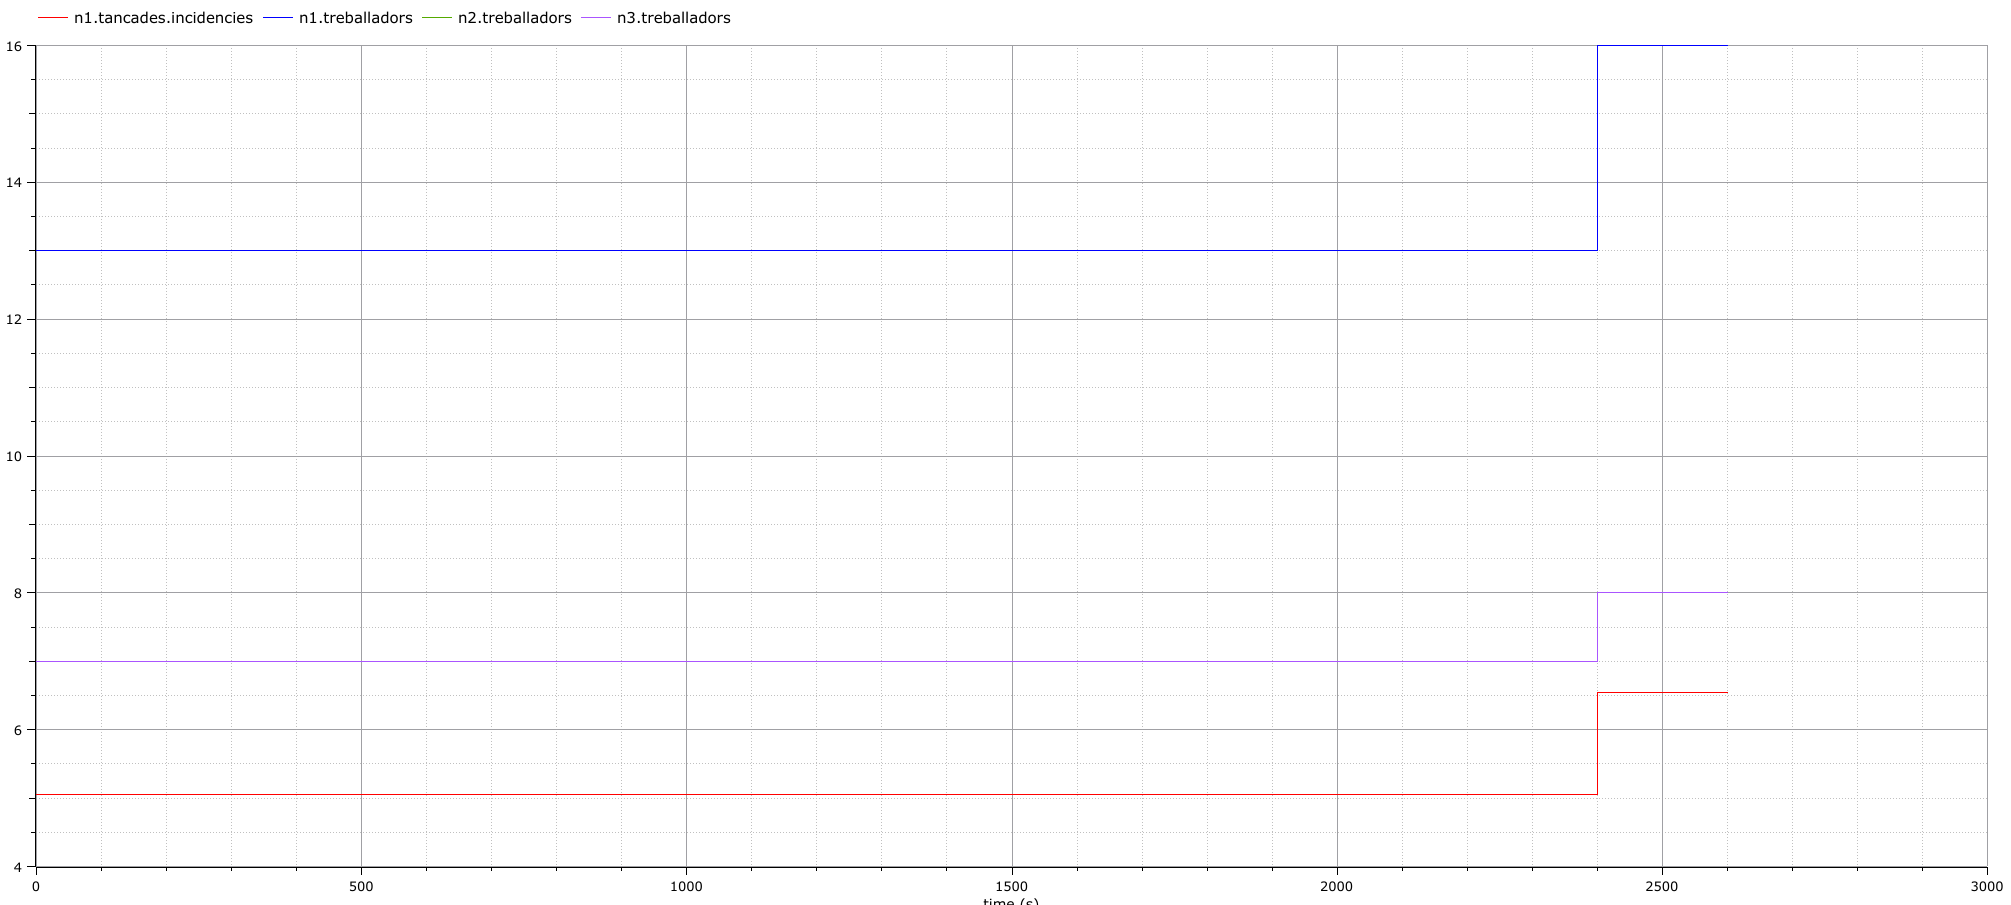
\includegraphics[width=\linewidth]{ex5.png}
  \caption{Gràfica dels treballadors per nivells (veure que els treballadors N2 i N3 es solapen)}
  \label{fig:plot1}
\end{figure}
\end{frame}
\begin{frame}
\subsection{Exercici 6}
\textbf{ Què passa si augmentem el nivell de formació del personal de Nivell 2 i el passem de 0.5
a 0.8? Quin serà el nou punt d’equilibri?}
\newline
\newline
El nou punt d'equilibri és 13 treballadors de nivell 1, 10 treballadors de nivell 2 i 3 treballadors de nivell 3.
\newline Al augmentar la formació dels treballadors hem passat de necessitar 27 treballadors en el supòsit original a 23.
\end{frame}
\begin{frame}
\subsection{Exercici 7}
\textbf{Què passa si augmentem el nivell de formació del personal de Nivell 1 en lloc del de Nivell
2 i el passem de 0.5 a 0.8? Quin serà el nou punt d’equilibri?}
\newline
\newline
El nou punt d'equilibri és 20 treballadors de nivell 1, 3 treballadors de nivell 2 i 3 treballadors de nivell 3.
\newline Continuem necessitant el mateix nombre de treballadors que en el supòsit anterior.
\end{frame}
\begin{frame}
\subsection{Exercici 8}
\textbf{Què passa si augmentem el nivell de formació del personal de Nivell 1 en lloc del de Nivell
2 i el passem de 0.5 a 0.8? Quin serà el nou punt d’equilibri?}
\newline
\newline
Si augmentem la formació dels usuaris i reduïm el número d'incidències generades a la meitat els usuaris tindràn una taxa d'indicències de 1/2000 incidències generades per persona i hora.
\newline El nou punt d'equilibri és de 7 treballadors de nivell 1, 4 treballadors de nivell 2 i 4 treballadors de nivell 3.
S'ha reduït el nombre de treballadors necessaris de 27 a 15.
\end{frame}
\end{document}